\documentclass[aspectratio=169,10pt]{beamer}

\usepackage[utf8]{inputenc}
\usepackage[T1]{fontenc}
\usepackage{tikz}
\usetikzlibrary{arrows.meta,positioning}
\usepackage{booktabs}
\usepackage{array}

\usetheme{default}
\setbeamertemplate{navigation symbols}{}
\setbeamertemplate{footline}[frame number]
\setbeamerfont{frametitle}{series=\bfseries}

\title{Leitura Automática de Displays de Multímetros\\com Detecção de Objetos (YOLO)}
\subtitle{Aplicações de Processamento Digital de Sinais -- Apresentação Inicial}
\author{Antônio \and Marcos \and Luige}
\date{10/11/2026}

\begin{document}

\begin{frame}
  \titlepage
\end{frame}

%% ------------------------------------------------------------------ problema
\begin{frame}{Problema}
  \begin{itemize}
    \item Calibração de multímetros portáteis: V$_\text{DC}$, V$_\text{AC}$,
          I$_\text{DC}$, I$_\text{AC}$ e resistência.
    \item 3 ou 6 pontos por faixa, $\geq 4$ ciclos $\Rightarrow$ 8 leituras por ponto.
    \item Hoje a leitura do display é \alert{visual}, feita pelo operador.
    \item Instável: registrar máximo e mínimo. Estável: duas leituras consecutivas.
  \end{itemize}
  \vspace{2mm}
  \textbf{Objetivo:} câmera fixa sobre o multímetro $\rightarrow$ ler, interpretar
  e registrar o valor automaticamente, para diferentes modelos de display.
\end{frame}

%% ----------------------------------------------------------------- abordagem
\begin{frame}{O que vamos fazer}
  \centering
  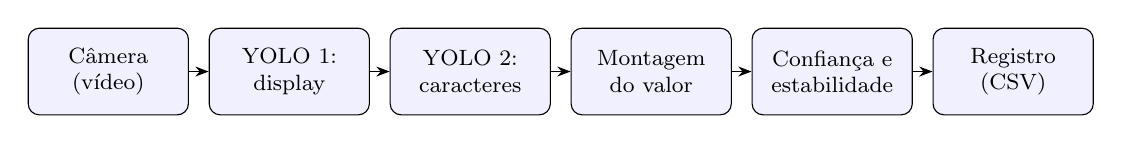
\begin{tikzpicture}[
      node distance=2.5mm,
      box/.style={draw, rounded corners, align=center, font=\footnotesize,
                  minimum height=11mm, text width=18mm, fill=blue!6},
      ->, >=Stealth]
    \node[box] (a) {Câmera\\(vídeo)};
    \node[box, right=of a] (b) {YOLO 1:\\display};
    \node[box, right=of b] (c) {YOLO 2:\\caracteres};
    \node[box, right=of c] (d) {Montagem\\do valor};
    \node[box, right=of d] (e) {Confiança e\\estabilidade};
    \node[box, right=of e] (f) {Registro\\(CSV)};
    \draw (a) -- (b); \draw (b) -- (c); \draw (c) -- (d);
    \draw (d) -- (e); \draw (e) -- (f);
  \end{tikzpicture}
  \vspace{3mm}
  \begin{enumerate}\small
    \item \textbf{YOLO 1} encontra o display no quadro e recorta.
    \item \textbf{YOLO 2} detecta cada caractere do recorte como uma classe:
          \texttt{0}--\texttt{9}, ponto decimal, sinal \texttt{-}, \texttt{OL}.
    \item Caracteres ordenados da esquerda para a direita; o ponto decimal
          define a posição da vírgula $\rightarrow$ número.
    \item Leitura com baixa confiança é descartada e o quadro seguinte é lido.
          Estável $\Rightarrow$ duas leituras consecutivas; oscilando $\Rightarrow$ máx. e mín.
    \item Cada leitura vai para o CSV com ponto, ciclo, horário e a imagem usada.
  \end{enumerate}
\end{frame}

%% ------------------------------------------------------------------- dados
\begin{frame}{Dados e avaliação}
  \begin{columns}[T]
    \begin{column}{0.48\textwidth}
      \textbf{Dados}
      \begin{itemize}\small
        \item Datasets públicos do Roboflow Universe, já anotados e
              exportáveis em formato YOLO:
          \begin{itemize}\footnotesize
            \item \textit{Multimeter Digits}: 779 imagens de multímetros.
            \item \textit{Seven segments display digits}: 13 classes
                  (\texttt{0}--\texttt{9}, \texttt{-}, \texttt{.}, \texttt{+}).
            \item \textit{7-Segment Display High Res}: classes
                  \textit{display} e \textit{led} (para o YOLO 1).
          \end{itemize}
        \item Unificação das classes entre os datasets.
        \item Aumento de dados: brilho, contraste, rotação, perspectiva,
              desfoque.
      \end{itemize}
    \end{column}
    \begin{column}{0.48\textwidth}
      \textbf{Avaliação}
      \begin{itemize}\small
        \item mAP de cada detector.
        \item \alert{Acerto da leitura completa}: valor inteiro correto,
              com ponto e sinal.
        \item Teste em modelos de multímetro \alert{fora do treino}.
        \item Taxa de rejeição: quantas leituras o sistema devolve ao operador.
      \end{itemize}
    \end{column}
  \end{columns}
\end{frame}

%% -------------------------------------------------------------- cronograma
\begin{frame}{Etapas e cronograma}
  \centering
  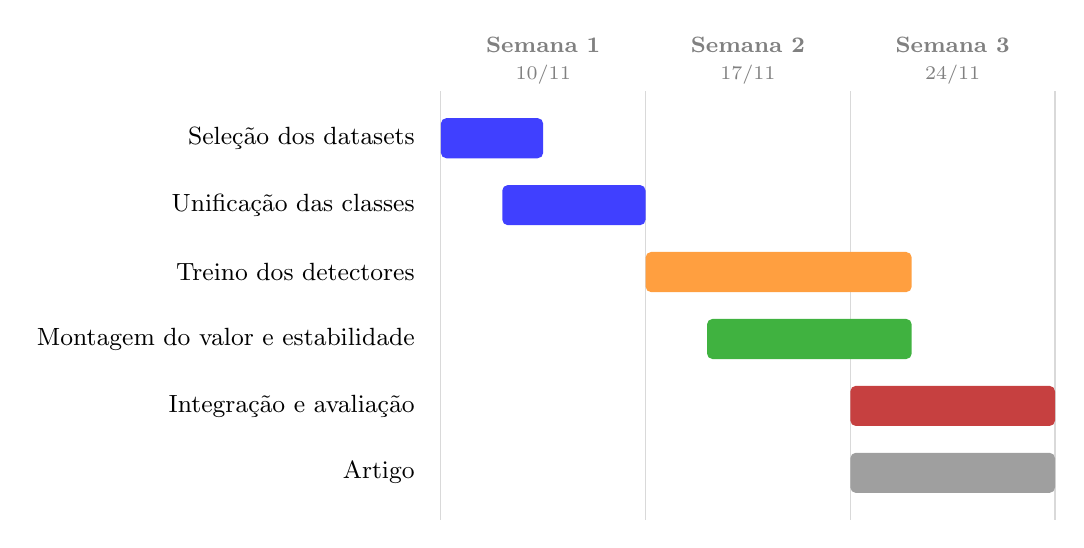
\begin{tikzpicture}[x=26mm, y=8.5mm, font=\small]
    \foreach \i/\d in {0/{10/11}, 1/{17/11}, 2/{24/11}} {
      \node[font=\footnotesize\bfseries, text=gray] at (\i+0.5, 0.9) {Semana \the\numexpr\i+1\relax};
      \node[font=\scriptsize, text=gray] at (\i+0.5, 0.45) {\d};
      \draw[gray!30] (\i, 0.2) -- (\i, -6.2);
    }
    \draw[gray!30] (3, 0.2) -- (3, -6.2);
    \foreach \y/\t/\a/\b/\clr in {
        1/Seleção dos datasets/0/0.5/blue,
        2/Unificação das classes/0.3/1/blue,
        3/Treino dos detectores/1/2.3/orange,
        4/Montagem do valor e estabilidade/1.3/2.3/green!60!black,
        5/Integração e avaliação/2/3/red!70!black,
        6/Artigo/2/3/gray} {
      \node[anchor=east, align=right] at (-0.08, -\y+0.5) {\t};
      \fill[\clr!75, rounded corners=2pt] (\a, -\y+0.2) rectangle (\b, -\y+0.8);
    }
  \end{tikzpicture}
\end{frame}

%% --------------------------------------------------------------- desafios
\begin{frame}{Principais desafios}
  \small
  \begin{tabular}{@{}>{\raggedright\arraybackslash}p{0.40\textwidth}
                    >{\raggedright\arraybackslash}p{0.54\textwidth}@{}}
    \toprule
    \textbf{Desafio} & \textbf{Como vamos tratar} \\
    \midrule
    Cada fabricante tem um display diferente
      & Treinar com o máximo de modelos possível e testar em modelos
        que ficaram fora do treino \\[1mm]
    Datasets com classes diferentes (alguns sem ponto ou sinal)
      & Mapear para um conjunto único de classes; completar a anotação
        onde faltar \\[1mm]
    Ponto decimal e sinal: um erro muda o valor em 10$\times$ ou inverte o sinal
      & Classes próprias no detector; leitura com baixa confiança é descartada \\[1mm]
    Display com vários campos (ex.: Fluke 789: leitura secundária, unidade, \textit{Manual Range})
      & Ler só a linha principal: a maior linha de caracteres detectada \\[1mm]
    Saber quando a leitura vale: LCD trocando de dígito, valor oscilando
      & Comparar quadros seguidos: estável $\Rightarrow$ duas leituras
        consecutivas; oscilando $\Rightarrow$ máx. e mín. \\
    \bottomrule
  \end{tabular}
\end{frame}

\end{document}
